% Stolen from: https://stackoverflow.com/questions/1603301/how-to-add-page-numbers-to-postscript-pdf
\documentclass[a4paper]{report}
\usepackage[final]{pdfpages}

\usepackage{fontspec}
\newfontfamily\unicodefont{Times New Roman}
\usepackage[T1]{fontenc}

\newcommand{\textcomma}{, }

\begin{document}

\thispagestyle{empty}

\mbox{}
\vspace{3cm}

\begin{center}
\begin{figure}[here]
\centering
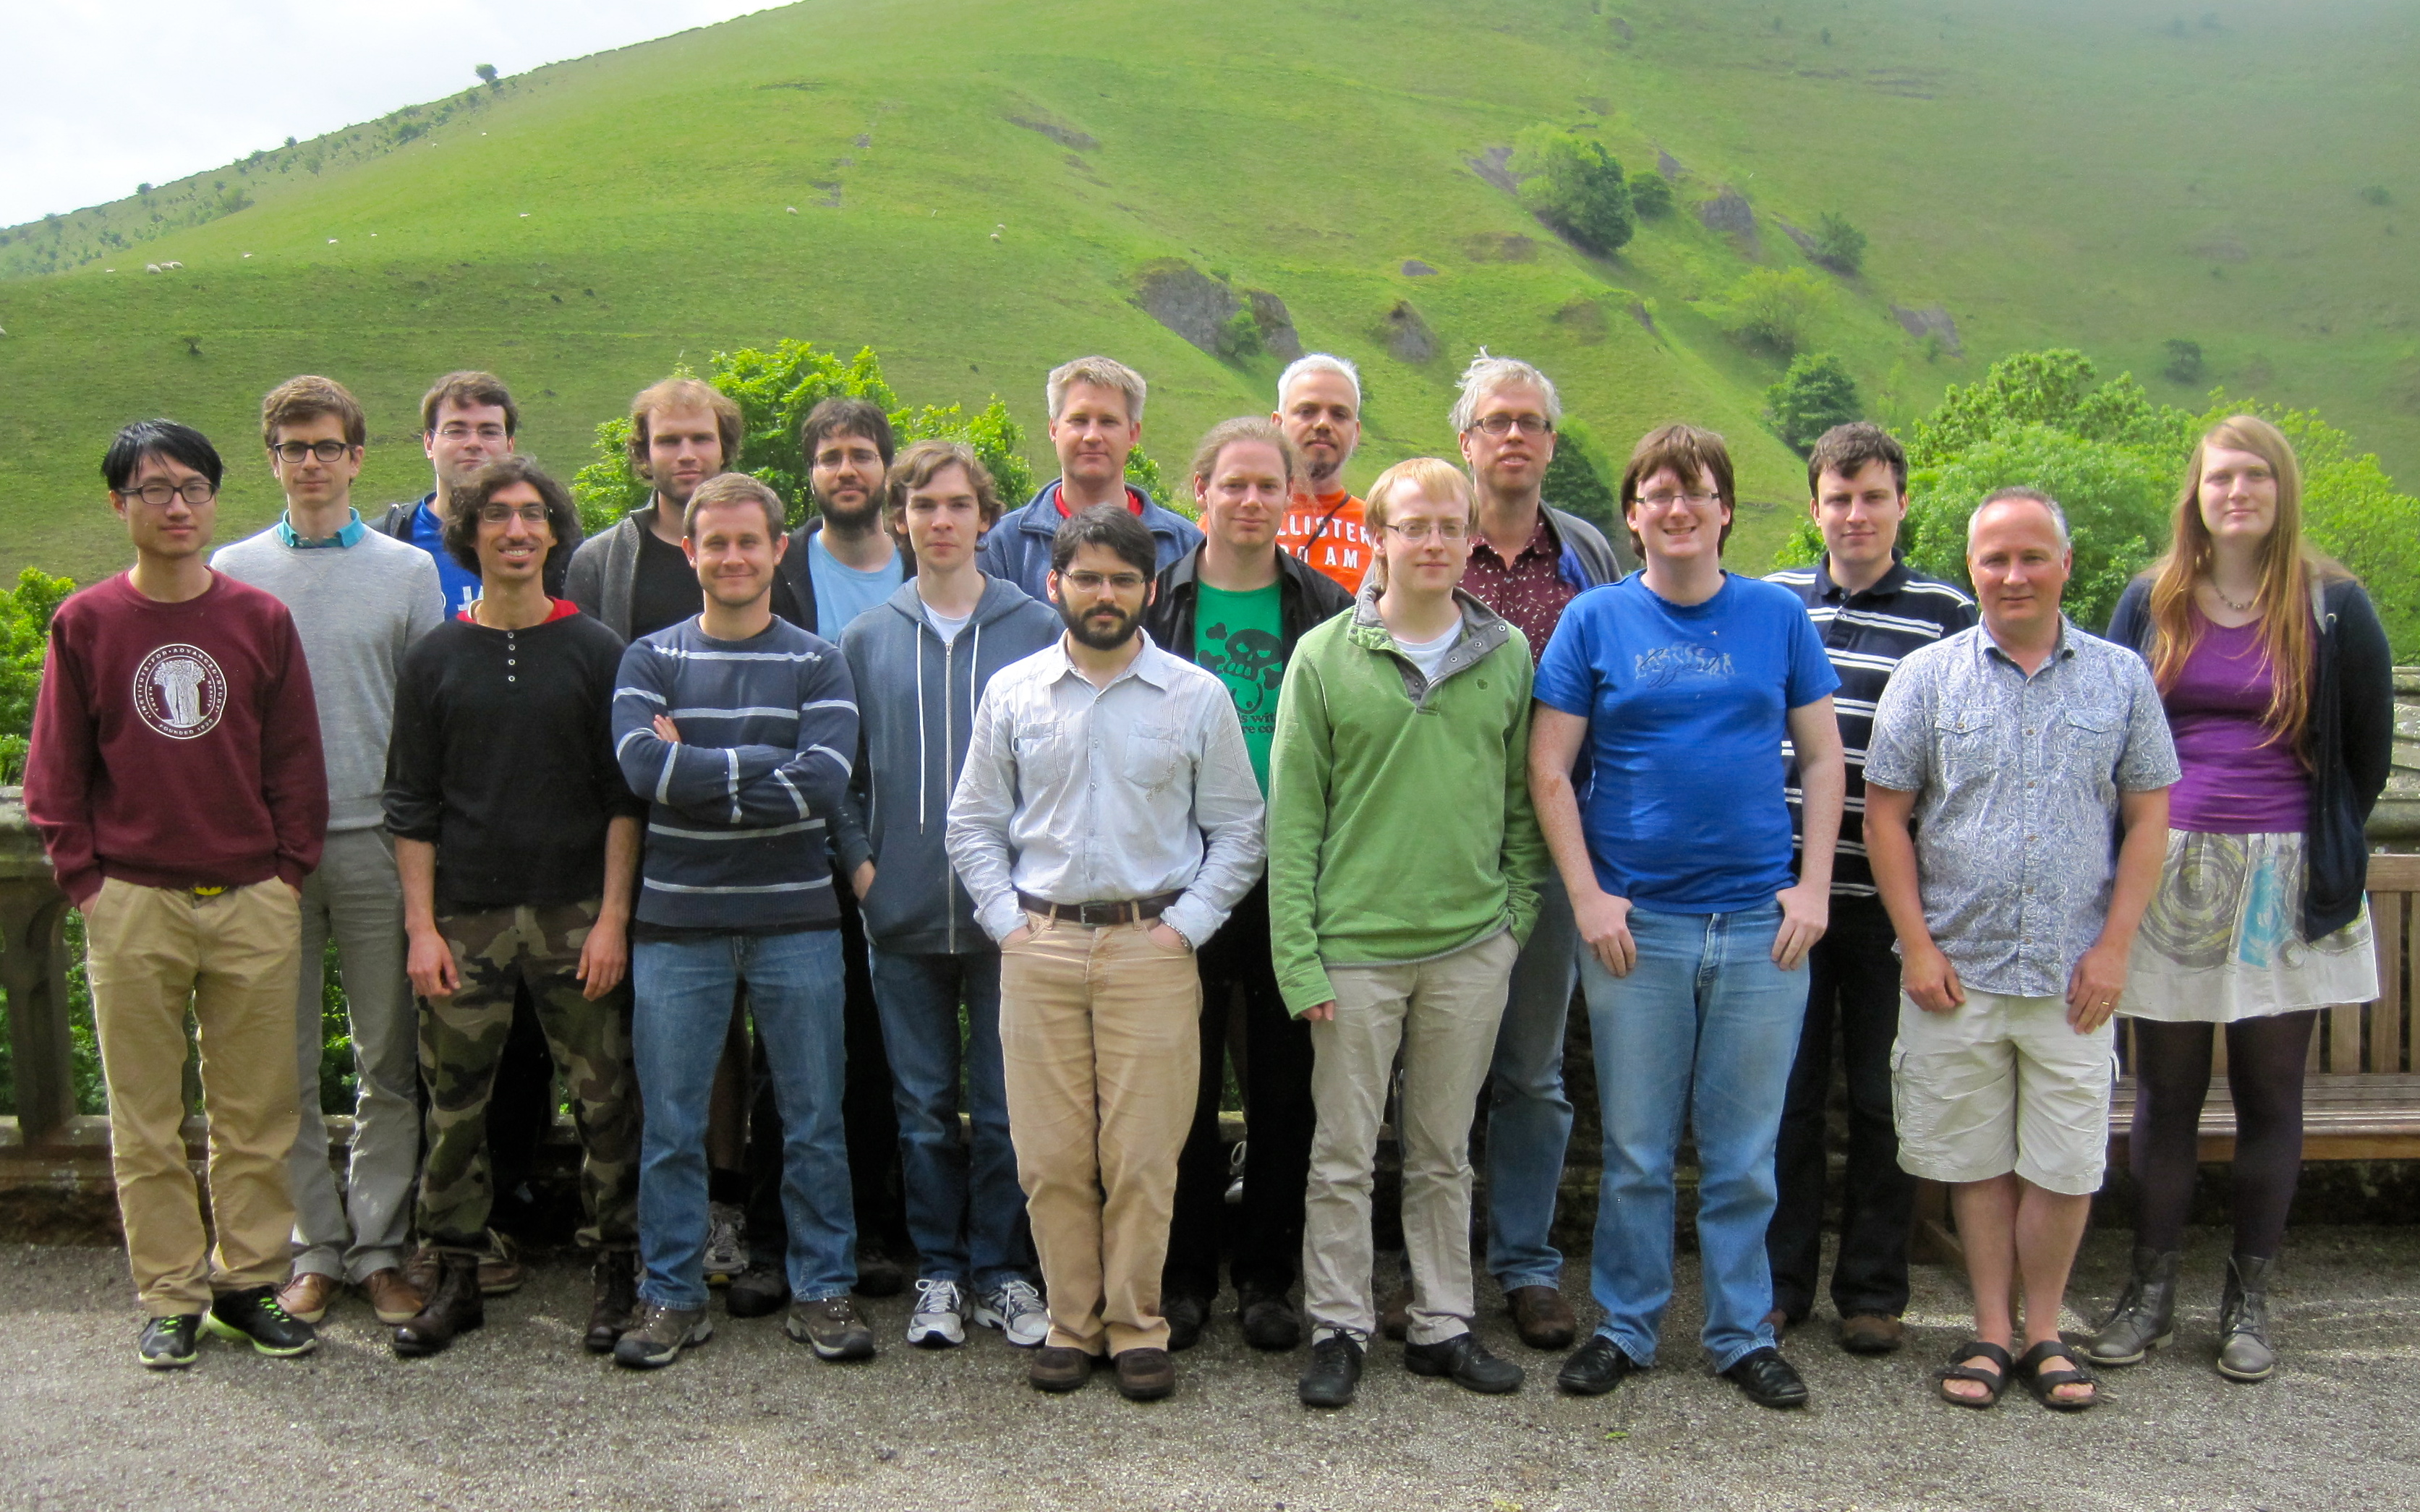
\includegraphics[width=12cm]{FP-LAB.jpg}
\end{figure}

Functional Programming Lab

The University of Nottingham

2014

\end{center}

\newpage

\tableofcontents

\newpage

\thispagestyle{empty}
\mbox{}

\newpage

% page number - 2, section, level, heading, label
\includepdfset{pages=-,pagecommand=\thispagestyle{plain},addtotoc={
  1,  chapter,0, \emph{Worker/Wrapper/Makes it/Faster}\\Jennifer Hackett and Graham Hutton                                                        ,p2,
  14, chapter,0, \emph{Calculating Correct Compilers}\\Patrick Bahr and Graham Hutton                                                             ,p15,
  38, chapter,0, \emph{Pick'n'Fix: Modular Control Structures}\\Laurence E. Day and Patrick Bahr                                                  ,p39,
  55, chapter,0, \emph{Attribute Grammars and Containers}\\Florent Balestrieri                                                                    ,p56,
  56, chapter,0, \emph{An Investigation Into the Use of Haskell for Dynamic Programming}\\David McGillicuddy\textcomma Andrew J. Parkes\textcomma Henrik Nilsson ,p57,
  62, chapter,0, \emph{EBBA: An Embedded DSL for Bayesian Inference}\\Henrik Nilsson                                                              ,p63,
  63, chapter,0, \emph{Extended Abstract: Bridging the GUI Gap with Reactive Values and Relations}\\Iv\'an P\'erez and Henrik Nilsson             ,p64,
  73, chapter,0, \emph{A principled approach to the implementation of argumentation models}\\Bas van Gijzel and Henrik Nilsson                    ,p74,
  81, chapter,0, \emph{Definability and Kripke Logical Relations}\\Thorsten Altenkirch                                                            ,p82,
  88, chapter,0, \emph{A syntax for cubical type theory}\\Thorsten Altenkirch and Ambrus Kaposi                                                   ,p89,
  109,chapter,0, \emph{Constructing 2-HITs}\\Gabe Dijkstra                                                                                        ,p110,
  125,chapter,0, \emph{Mutual and Higher Inductive Types in Homotopy Type Theory}\\Paolo Capriotti                                                ,p126,
  142,chapter,0, \emph{Omega-Constancy and Truncations}\\Nicolai Kraus                                                                            ,p143,
  150,chapter,0, \emph{Definable quotients in intensional type theory}\\Nuo Li                                                                    ,p151
}}
\includepdf{papers.pdf}


\end{document}
